% \documentclass{standalone}
% \usepackage[usenames, dvipsnames, table, tikz]{xcolor}
% \usepackage{tikz}
% \begin{document}
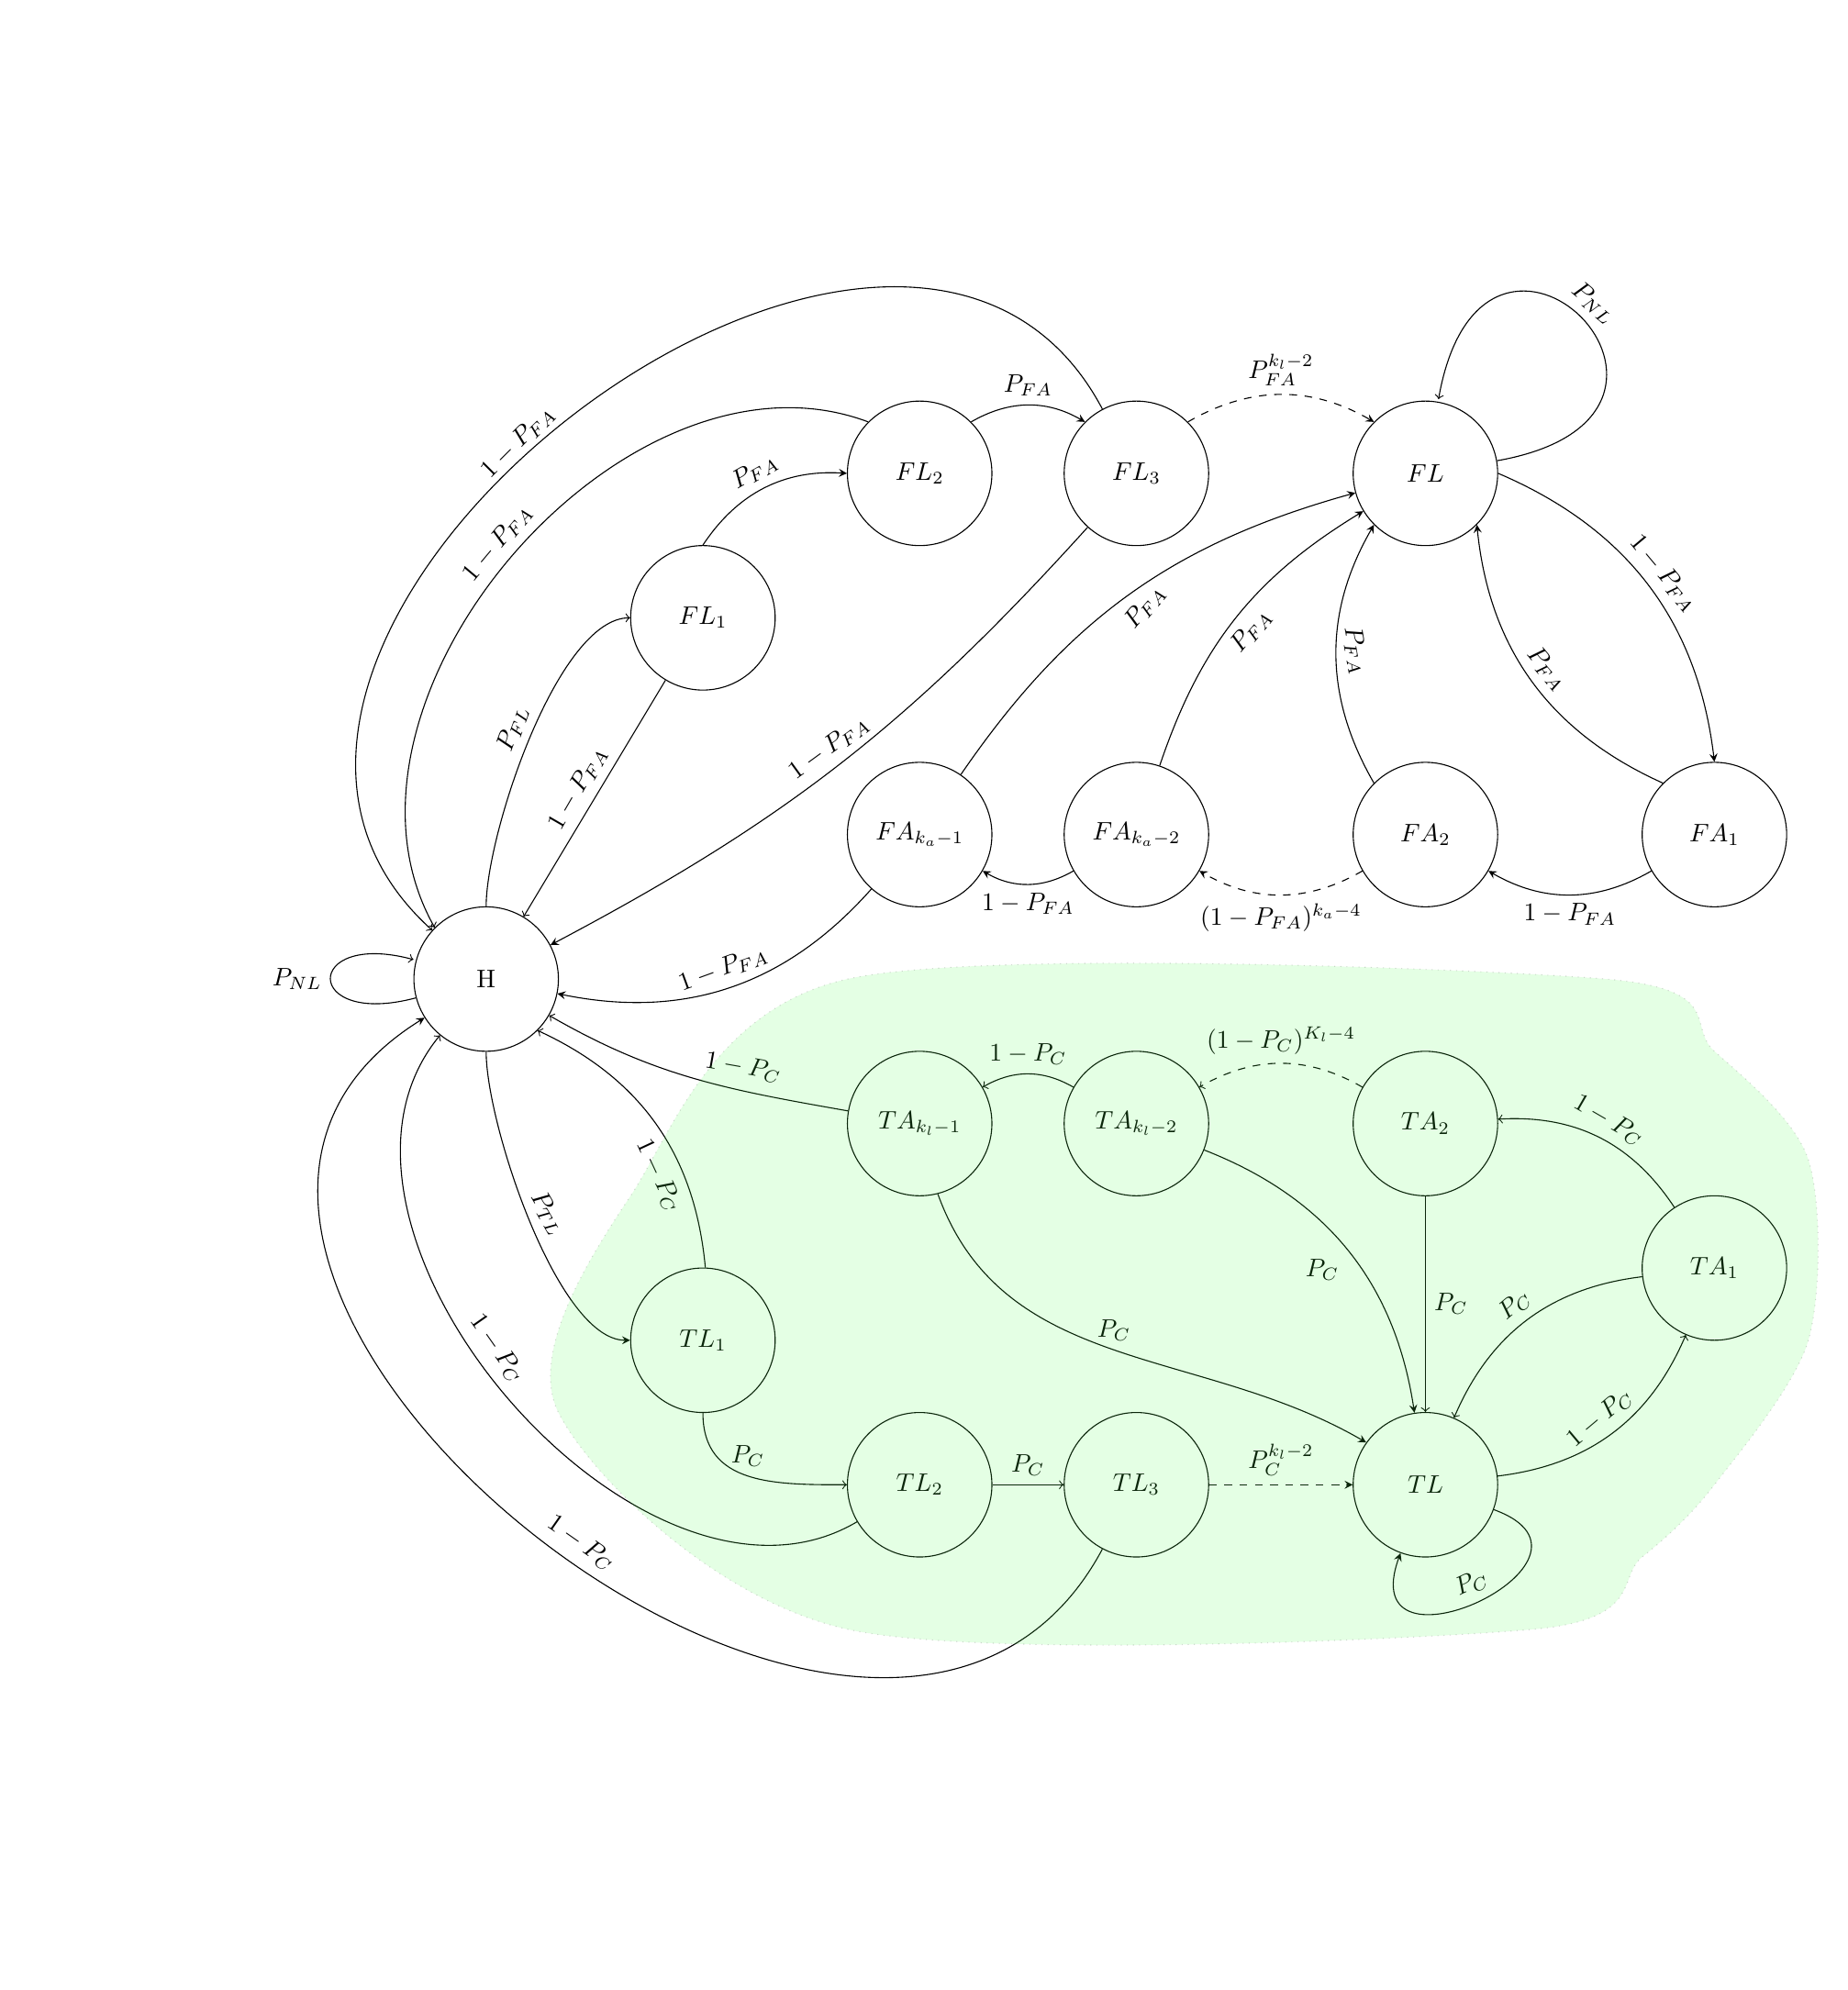
\begin{tikzpicture}
  [
    my circle/.style={minimum width=20mm, circle, draw},
    my label/.style={above=10pt, anchor=mid}
  ]
  \node[my circle] (H) at (-15,0) {H};
  \node[my circle] (fl1) at ( -12,5) {$FL_1$};
  \node[my circle] (tl1) at ( -12,-5) {$TL_1$};
  \node[my circle] (faKa1) at ( -9,2) {$FA_{k_a-1}$};
  \node[my circle] (fl2) at ( -9,7) {$FL_2$};
  \node[my circle] (taKa1) at ( -9,-2) {$TA_{k_l-1}$};
  \node[my circle] (tl2) at ( -9,-7) {$TL_2$};
  \node[my circle] (faKa2) at ( -6,2) {$FA_{k_a-2}$};
  \node[my circle] (fl3) at ( -6,7) {$FL_3$};
  \node[my circle] (taKa2) at ( -6,-2) {$TA_{k_l-2}$};
  \node[my circle] (tl3) at ( -6,-7) {$TL_3$};
  \node[my circle] (fa1) at ( 2,2) {$FA_1$};
  \node[my circle] (fa2) at ( -2,2) {$FA_2$};
  \node[my circle] (fl) at ( -2,7) {$FL$};
  \node[my circle] (ta1) at ( 2,-4) {$TA_1$};
  \node[my circle] (ta2) at ( -2,-2) {$TA_2$};
  \node[my circle] (tl) at ( -2,-7) {$TL$};

  %\path [postaction={draw, {>[sep=5pt,reversed]}-{<[sep=5pt]}}, draw] (1) -- (2) node [very near start, my label] {$a$}  node [very near end, my label] {$\beta$} ;
  %
  % --- PATH INVOLVING H ---
  %
  \path[-stealth] (H) edge[loop left]  node{$P_{NL}$} (H);
  \draw[-stealth] (H.south) .. controls +(down:1cm) and +(left:1cm) .. node[above,rotate=-60] {$P_{TL}$} (tl1.west);
  \path[->] (tl1) edge[bend right] node[below right, rotate=-65] {$1-P_{C}$}  (H.south east);
  \draw[->] (H.north) .. controls +(up:1cm) and +(left:1cm) .. node[above,rotate=70] {$P_{FL}$} (fl1.west);
  \path[->] (fl1) edge[bend right,out=0,in=180] node[above, rotate=60] {$1-P_{FA}$}  (H);
  \path[->] (fl2.north west) edge[bend right =70] node[above, rotate=50] {$1-P_{FA}$}  (H.north west);

  %
  % --- PATH INVOLVING TL# ---
  %
  \draw[->] (tl1.south) .. controls +(down:1cm) and +(left:1cm) .. node[above] {$P_C$} (tl2.west);

  \draw[->] (tl2.east) .. controls +(right:1cm) and +(left:1cm) .. node[above] {$P_C$} (tl3.west);

  \path[->] (tl2) edge[bend left,in=100,out=80,min distance=0.3cm] node[above left, rotate=-55] {$1-P_C$} (H);

  \draw[-stealth,dashed] (tl3.east) .. controls +(right:1cm) and +(left:1cm) .. node[above] {$P_C^{k_{l}-2}$} (tl.west);
  \path[-stealth] (tl3) edge[bend left,in=70,out=100,min distance=6.5cm] node[above right, rotate=-35] {$1-P_C$} (H);
  \path[-stealth] (tl) edge[in=-110, out=-20,min distance=2cm]  node[above,rotate=25]{$P_{C}$} (tl);
  %
  % --- PATH INVOLVING TA# ---
  %
  \path[->] (tl) edge[bend right] node[above, rotate=40] {$1-P_C$} (ta1);
  \path[->] (ta1) edge[bend right] node[above, rotate=40] {$P_C$} (tl);
  \path[->] (ta1) edge[bend right] node[above, rotate=-30] {$1-P_C$} (ta2);
  \path[->] (ta2) edge[] node[right, rotate=0] {$P_C$} (tl);
  \path[->,dashed] (ta2) edge[bend right] node[above, rotate=0] {$(1-P_C)^{K_l-4}$} (taKa2);
  \path[-stealth] (taKa2) edge[bend left] node[below left, rotate=0] {$P_C$} (tl);
  \path[->] (taKa2) edge[bend right] node[above, rotate=0] {$1-P_C$} (taKa1);
  \path[-stealth] (taKa1) edge[bend right, in=180,out=-40] node[above, rotate=0] {$P_C$} (tl);
  \path[->] (taKa1) edge[in=-30,out=170] node[above right, rotate=-10] {$1-P_C$} (H);
  %
  % --- PATH INVOLVING FL# ---
  %
  \path[-stealth] (fl1.north) edge[bend left] node[above,rotate=30] {$P_{FA}$}  (fl2.west);
  \path[-stealth] (fl2.north east) edge[bend left] node[above,rotate=0] {$P_{FA}$}  (fl3.north west);
  \path[-stealth] (fl3) edge[bend left, in=-190,out=10] node[above,rotate=36] {$1-P_{FA}$}  (H);
  \path[-stealth,dashed] (fl3.north east) edge[bend left] node[above,rotate=0] {$P_{FA}^{k_l-2}$}  (fl.north west);
  \path[-stealth] (fl) edge[in=80, out=10, loop]  node[above,rotate=-40]{$P_{NL}$} (fl);
  \path[-stealth] (fl.east) edge[bend left] node[above,rotate=-50] {$1-P_{FA}$}  (fa1.north);
  \path[-stealth] (fa1.north west) edge[bend left] node[above,rotate=-50] {$P_{FA}$}  (fl.south east);
  \path[->] (fl3) edge[bend left ,out=260,in=-80,min distance=6cm] node[above left, rotate=45] {$1-P_{FA}$} (H);


  %
  % --- PATH INVOLVING FA# ---
  %
  \path[-stealth] (fa2.north west) edge[bend left] node[above,rotate=-80] {$P_{FA}$}  (fl.south west);
  \path[-stealth] (fa1) edge[bend left] node[below] {$1-P_{FA}$}  (fa2);
  \path[-stealth,dashed] (fa2) edge[bend left] node[below] {$(1-P_{FA})^{k_a -4}$}  (faKa2); %verify formula. not sure
  \path[-stealth] (faKa2) edge[bend left] node[below] {$1-P_{FA}$}  (faKa1);
  \path[-stealth] (faKa1) edge[bend left] node[above,rotate=20] {$1-P_{FA}$}  (H);
  \path[-stealth] (faKa2) edge[bend left,in=-200,out=20] node[below, rotate=50] {$P_{FA}$}  (fl);
  \path[-stealth] (faKa1) edge[bend left,in=-200,out=20] node[below, rotate=50] {$P_{FA}$}  (fl);

  %Final line where I'd like to be
  \draw[dotted,fill=green!70, opacity=0.15] plot [smooth cycle] coordinates {(3.3,-2.5) (3.3,-5) (2,-7) (1,-8) (-0.5,-9) (-10,-9) (-14,-6) (-13,-3) (-10,0) (0.5,0) (2,-1)};

\end{tikzpicture}
% \end{document}
